\documentclass{mcmthesis}
\mcmsetup{CTeX = false,
        tcn = 2109976, problem = C,
        sheet = true, titleinsheet = true, keywordsinsheet = true,
        titlepage = true}
\usepackage{palatino}
\usepackage{mwe}
\usepackage{graphicx}
\usepackage{subcaption}
\usepackage{float}
\usepackage{multirow}
\usepackage{indentfirst}
\usepackage{gensymb}
\usepackage[ruled,lined,commentsnumbered]{algorithm2e}
\usepackage{diagbox}

\usepackage{geometry}
\geometry{left=2cm,right=2cm,top=2cm,bottom=2cm}
\begin{document}
\linespread{0.6}
\setlength{\parskip}{0.5\baselineskip}
\title{Title}

\date{\today}
\begin{abstract}

We construct two neural-network-based models to resolve the problems of Vespa mandarinia spread situation and identification of the pest by images. We make several hypotheses to simplify the issues. For instance, we assume that the sightings are related in both dimensions, time and space, to make neural network applicable for the problems. Also, the living conditions are considered as similar to the natural pattern as the past to avoid outside disturbance. After investigating several models, we finalize that the long short-term memory (LSTM) model is to solve the problems of prediction while another model based on deep neural network (LSTM) is to solve the issue of classification.

Firstly, LSTM is a special branch of recurrent neural network (RNN). Traditionally, RNN is used to solve short-term dependencies problems. Its performance is not good when dealing with long-term dependencies problems which characteristics long time lag connection. The prediction of spread situation of Vespa mandarinia is a typical long-term dependencies problem. There are thousands of discrete reports of sightings distributed unevenly in a time span over one year. Consequently, we choose LSTM instead of RNN to resolve this problem. Then we divide the useful data into two main groups. The larger part is used as train set while the other one is used as testing set. Then LSTM model is developed to able to predict the spread situation in the future.

Furthermore, confronting the problem of classification of images, the first thought we have is to use logistic regression. It is because that the result of classification of images can only be two, it is or is not a Vespa mandarinia. As a consequence, the statistics will follow a binomial distribution. Then, what we consider is the classification problem. Neural network is a common method to identify and classify images with a lot of parameters. Due to the quantity of given pictures, we choose to use a deep 5-layer-neural network. With the pixels as input, the model will learn the characteristics of Vespa mandarinia in the pictures and will be able to classify a new image by judging if there are Vespa mandarinia within.

In conclusion, our models can be of use in predicting the spread situation and classify images by the existence of Vespa mandarinia. Moreover, by processing the results of the prediction model, we can obtain the knowledge of the distribution of locations of potential positive ID sighting. Such information will be of help in increasing the working efficiency of the relevant government department by prioritizing sightings with higher possibility to be positive ID. The dominant advantage of our model is its high accuracy, which is nearly 90\% for the classification model. Though there are still some weaknesses such as the relative slow computing speed, there are lots of space for our model to be improved and updates. 

	\begin{keywords}
	LSTM, Deep neural network,keywords3
	\end{keywords}
\end{abstract}

\maketitle

\tableofcontents
\newpage

\section{Introduction}

\subsection{Problem statement}
Vespa mandarinia was witnessed in Washington State since the discovery of the pest in the adjacent region of Canada in September 2019. In total, 4440 sighting incidents took place in the following year. Only 14 sightings was confirmed as witnesses of Vespa mandarinia while thousands of cases were mistaken or cannot be verified without adequate information. Therefore, a problem arose. Compared to the numerous reported sightings, the state government agencies with limited power may not draw timely validated conclusions to the incidents. Moreover, the lack of efficiency in identifying the right species would lead to a imprecise or useless model for the spread of Vespa mandarinia.

The reason why the government needs to identify the Vespa mandarinia and figure out how it spreads in the district is that it is harmful for the local species, especially honeybees. Vespa mandarinia is also known as the Asian giant hornet. More specifically, we learn that it is the largest species of hornets across the world, originating in the tropical region of eastern Asia. As an alien species to the state, Vespa mandarinia not only occupies some local natural resources, but invades the native European honeybees. Its invasion activity reaches the peak in September and October when the population of a single colony also becomes the largest in a year \cite{AGH}.

In order to fulfill the requirement, we developed a model that can predict the spread situation of Vespa mandarinia based on reported sightings. Then with the given images, we derived a model to predict the correctness of classification. Finally, our model can be further improved with increasing sightings and be of use in reality.



\subsection{Assumptions}
\subsubsection{Assumptions for the Prediction Model}
\begin{itemize}
    \item All the sightings that are positively identified are relevant in both dimensions of time and space.
    \item The cases before 2019 can be considered as irrelevant to the discovery of Vespa mandarinia in Canada and the Washington State in 2019 and 2020.
    \item The Vespa mandarinia found in the Washington State from 2019 to 2020 came from one incidents of invasion of alien species.
    \item Since the time when Vespa mandarinia was first found in the Washington State in 2019, the biological habits of the pest, including the breeding habits, retained unchanged.
    \item The unverified sightings are considered as positive identification.
\end{itemize}

\subsubsection{Assumptions for the Classification Model}
\begin{itemize}
    \item Vespa mandarinia can be identified by its appearance.
    \item From 2019 to 2020, the appearance of Vespa mandarinia in the district is inhabited stably.
    \item The species of Vespa mandarinia in the district is only one kind and each has alike appearance.
    \item The local species have not developed highly similar appearances as Vespa mandarinia. 
\end{itemize}




\section{Model Construction}

\subsection{Prediction Model}
\subsubsection{Brief of Long Short-term Memory}
Long short-term memory (LSTM) was developed to solve the long-term dependencies problems that usually have extended time lags in recurrent neural network (RNN). Take the identification of image as an example as an instance, ordinary RNN can predict that one pixel is blue if and only if a number of surrounding pixels are all blue, while LSTM can predict the color of a pixel by the information obtained previously or even far ago. For example, if the previous identified part of image has the mirror characteristic, LSTM model can predict that the next pixel may have the same color with the corresponding pixel by symmetry. LSTM performs well when dealing with long-term dependencies problems.
Consequently, LSTM is the model that we use to predict the spread situation of Vespa mandarinia.
\subsubsection{Notations}
The notations used in the following part are listed in the table Tab. 1.

\begin{table}[htbp]
\centering
\begin{tabular}{lll}
\hline 
Symbol & Definition & Comments \\
\hline
$f_{\text {t }}$ & the forget information determinant & \\
$\sigma$ & the sigmoid neural network & varies from 0 to $1$ \\
$W_{f}$ & the slope of regression & similar to $W_{i} $ and $W_{o}$\\
$h_{t-1}$ & the signal from the previous block & \\
$x_{t}$ & the input information at current block & \\
$b_{f}$ & a linear coefficient & same as $b_{i}$ and $b_{C}$\\
$i_{t }$ & the input information determinant &  \\
$\tilde{C_{t }}$ & the candidate vector &  \\
$o_{t }$ & the output information determinant &  \\
$h_{t }$ & the signal that generates in the current block &  \\
$C_{t }$ & the current cell status  &  \\
\hline
\label{tab:1}
\end{tabular}
\caption{Notations}
\end{table}

\subsubsection{Structure of LSTM}
Due to the special settings of LSTM blocks, this model is suitable for processing and predicting the data in a time sequence that are separated extensively. Here is the scheme of LSTM fig.~\ref{fig:LSTM}.

\begin{figure}[!htbp]
	\centering
 	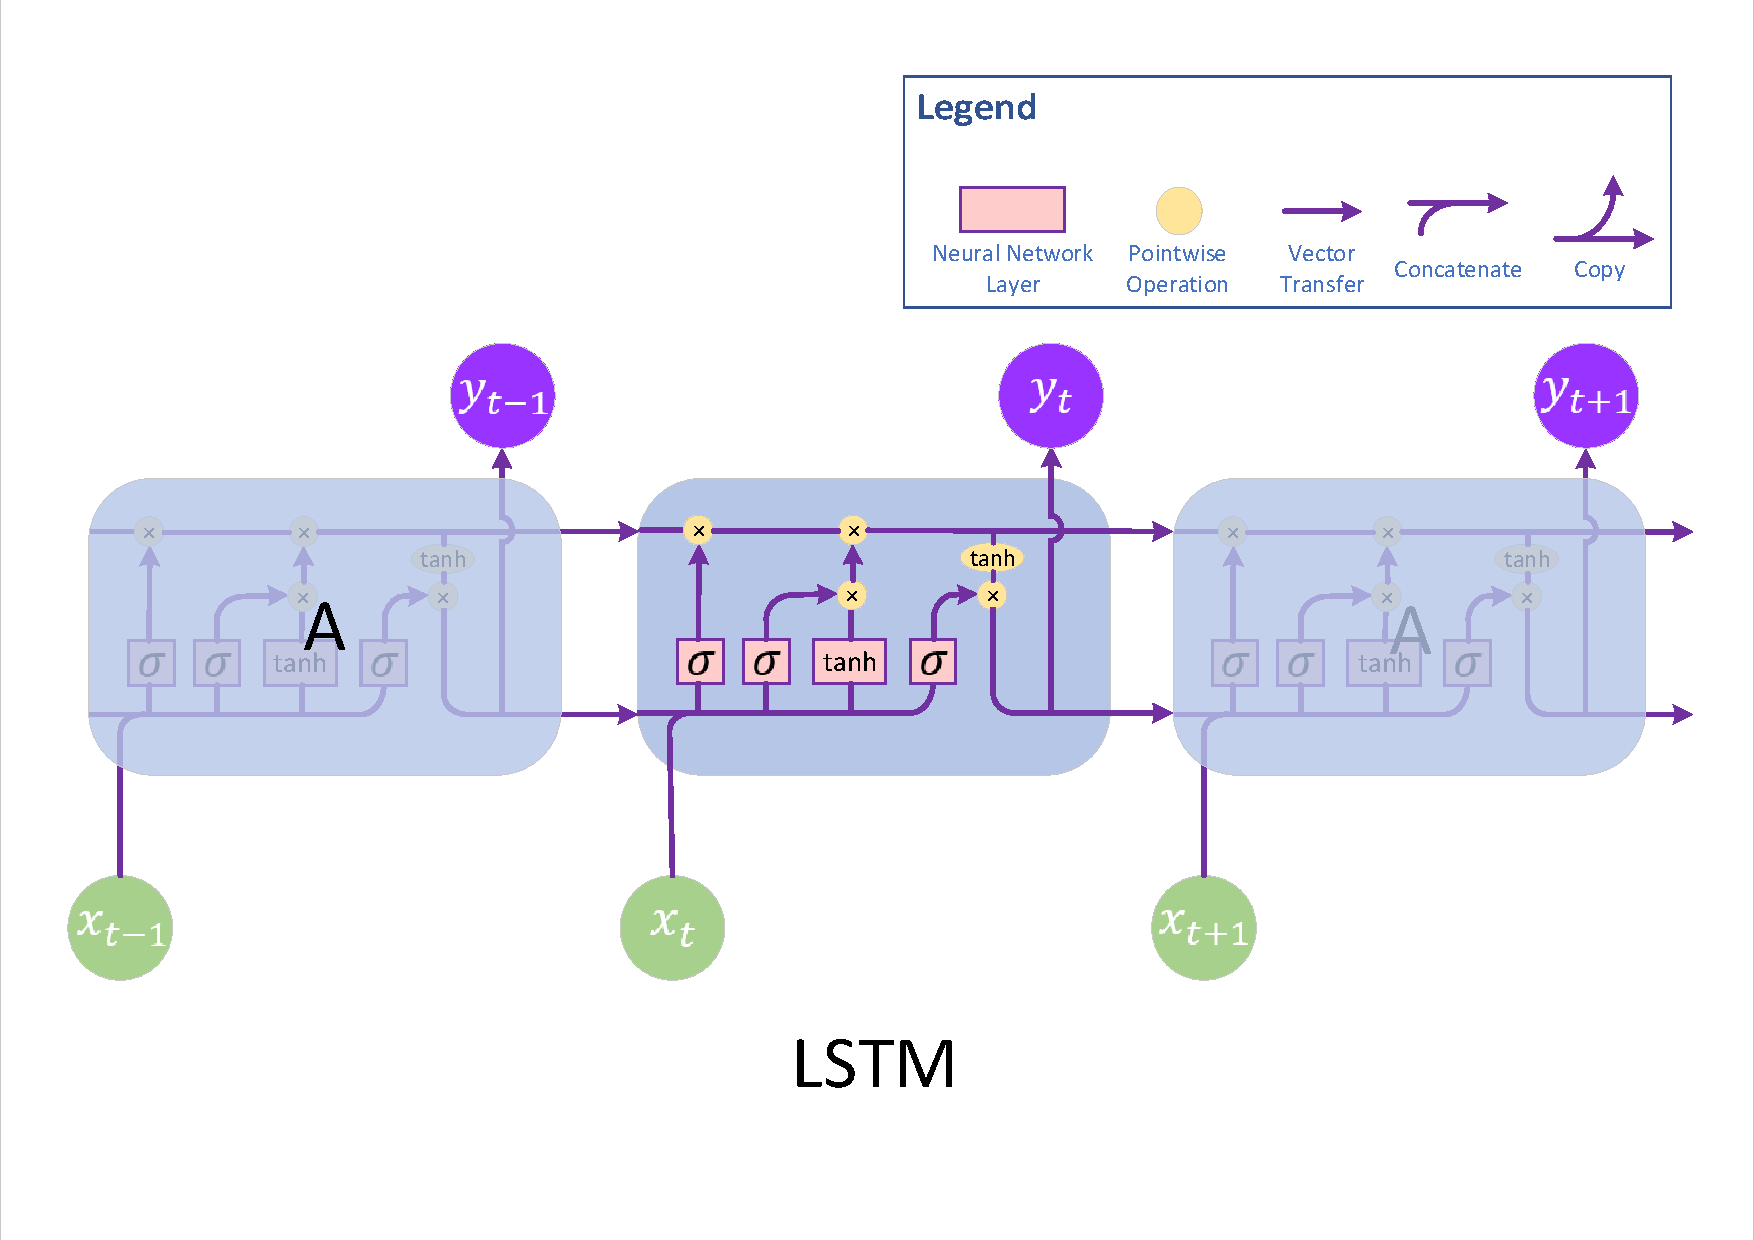
\includegraphics[width = 0.7\textwidth]{LSTM.pdf} 
	\caption{Basic Structure of LSTM}
	\label{fig:LSTM}
\end{figure}

The upper horizontal line is the kernel of LSTM, the cell status. It's like the carrying belt in a factory. The goods it carries is information and the machine arms that add or take the goods away are called gates. The gates are composed of a sigmoid layer, which can output a number varying from 0 to 1, proportional to the amount of information that is allowed to pass, and a bitwise multiplicative operation. There are in total three kinds of gates in LSTM, which are forget gate, input gate and output gate. They are used to change and protect the cell status \cite{LSTM}.

\paragraph{Forget Gate}
The first and most important step of a LSTM is to determine what to forget or drop from the cell status. This function is achieved by the forget gates. For example, when identifying an image, it detects a new block of pixels with the same color, the previous color ought to be forgotten and predict the present color with the only information from the nearby area. When the computer process this, it computes the value of $\sigma$ by
\begin{equation}
	f_{t}=\sigma(P_{f}\cdot [h_{t-1}, x_{t}]+b_{f}).
\end{equation}
Then a value varying from 0 to 1 will represents the amount of information that is retained. 0 means totally discard while 1 implies retain all.

\paragraph{Input Gate}
The next step is to determine what to add to the cell status. The sigmoid neural network will determine what values to update and a $tanh$ layer will create a new candidate vector. Then, the generation of such information will cause the update of the cell status. Still the case of image identification. The color of nearby pixels should be added to replace the previous color and then the prediction can be made. This update process can be described by the following formula.
\begin{equation}
	i_{t}=\sigma(P_{f}\cdot [h_{t-1}, x_{t}]+b_{i}).
\end{equation}

\begin{equation}
	\tilde C_{t}=\text{tanh}(P_{C}\cdot [h_{t-1}, x_{t}]+b_{C}).
\end{equation}
After updating the information, it should be added to update the cell status.
\begin{equation}
	C_{t}=f_{t}*C_{t-1}+i_{t}*\tilde C_{t}
\end{equation}
\paragraph{Output Gate}
After updating the cell status, the block will output a value based on the current cell status. This process is done in two steps. First, we run a sigmoid layer to determine which part of the cell status is to be output. The result of this step is calculated by Eq. (5). Then, $o_{t}$ is multiplied by a tanh. Finally, the output signal is determined by Eq. (6).
 \begin{equation}
	o_{t}=\sigma(W_{o}\cdot [h_{t-1}, x_{t}]+b_{o}).
\end{equation}
\begin{equation}
	h_{t}=o_{t}*tanh(C_{t})
\end{equation}

From the analysis above, we learn that LSTM is suitable for predicting the spread situation of Vespa mandarinia, which is a typical long-term dependencies problem.

\subsubsection{Introduction of LSTM to the Real Case} 
The real case we were to deal with is to predict the spread situation of Vespa mandarinia with given sightings in 2019 and 2020, merely with 14 positive identification cases reported out of 4440 cases in total. With such a complicated data set, the first thing we did was the data cleaning. All the cases that were proved not to be the sightings of Vespa mandarinia (negative ID) and those were not processed were deserted. 

The data we used were those positive ID and unverified cases. Then wed use a part them as the primary input of LSTM. Attention should be called here because one of the ordinary points of our model was to use only the cases before October in 2020, instead of all the cases. The aim was to separate the data  deliberately as a train set and a testing set. The data before October in 2020 were used to train the LSTM to predict the spread situation of Vespa mandarinia till the end of 2020. 

Once we obtained the prediction data, the testing set would be compared with the prediction set with feedback to the LSTM. With changing parameters, the error between the prediction set and the testing set would be minimized. The prediction results compared favorably with the testing data. At last, our model was constructed and was able to predict the future spread situation of Vespa mandarinia. More details of the results will be discussed in the Simulation Results Section.


\subsection{Classification Model}

\subsubsection{Brief of Deep Neural Network}
Given an image of a reported sighting, there are two possibilities, the animal in the image is a Asian Giant Hornet or not an Asian Giant Hornet . The assumption is that for a given picture of a reported sighting, which is regarded as in put X, the corresponding Y, which indicates weather or not it's an Asian Giant Hornet (1 for true and 0 for flase) follows a binomial distribution. To predict whether a new reported sighting is credible, we can use Logistic Regression to calculate the value of the possibility that the creature in the picture is an Asian Giant Hornet. The model can be explained by Eq.(7)
\begin{equation}
    P(Y=1|X) = \frac{exp(\omega X)}{1 + exp(\omega X)} 
\end{equation} \label{logistic}
However, after applying the model we found out that the accuracy of this model is not high enough, which means we need more parameters in the model to increase the accuracy of our model. 
Neural Network is often used for classification due to the large number of parameters, and also its accuracy. So we used a deep neural network with five layers to predict the possibility that a picture is an Asian Giant Hornet.
\paragraph{ } The Neural Network accept an input of an image with size m * n * 3 where n and m is the resolution of the image and 3 means the picture is of mode "RGB" and the neural network will randomly initialize the parameters and calculate the value of Loss function which is shown by Eq.(8) in each iteration, then use back-propagate algorithms to 
get the gradient of each parameters and update the parameters along its gradient to find the minimum of the values of loss function.
\begin{equation}
    Loss = - \frac{1}{m} \sum_{i=1}^m (y*log(a^{[L]})+(1-y)*log(1-a^{[L]}))
\end{equation}
In this equation, y is the label of the picture and a is the input of some layer.
After we finished training the neural network, for another reported sighting, we can calculate its possibility of being a credible sighting as well as predicts the likelihood of a mistaken classification.
\subsubsection{Notations}
The notations used in the following part are listed in the table Tab. 2.

\begin{table}[htbp]
\centering
\begin{tabular}{lll}
\hline 
Symbol & Definition & Comments \\
\hline
$X_i$ & the i th image in the data set & \\
$y_i$ & whether the i th image is Vespa mandarinia & \\
$ \hat{y_i}$ &  prediction of whether the i th image is Vespa mandarinia & \\
$\sigma $ & the sigmoid function & varies from 0 to $1$ \\
$ReLU$ & Rectified Linear Unit \\
$a_{i}^{[L]}$ & the input in L th hidden layer for i th image & \\

$\omega, b$ & the parameters of the neural network &  \\
\hline
\label{tab:2}
\end{tabular}
\caption{Notations}
\end{table}

\subsubsection{Structure of Deep Neural Network}

In our Deep Neural Network model, there are five layers, the input layer, output layer and three hidden layers. The scale of input layer is 250 * 250 * 3 and output is 1, the reason is that we resized the pictures in the reported sightings to 250 * 250 and each picture can be splitted into three matrix representing the value of R, G, and B, and the output is just the possibility with size 1. The size of the three hidden layers are 20, 7, 5 separately. The structure of the deep neural network is shown in the figure fig.\ref{fig:DNN}

\begin{figure}[!htbp]
	\centering
 	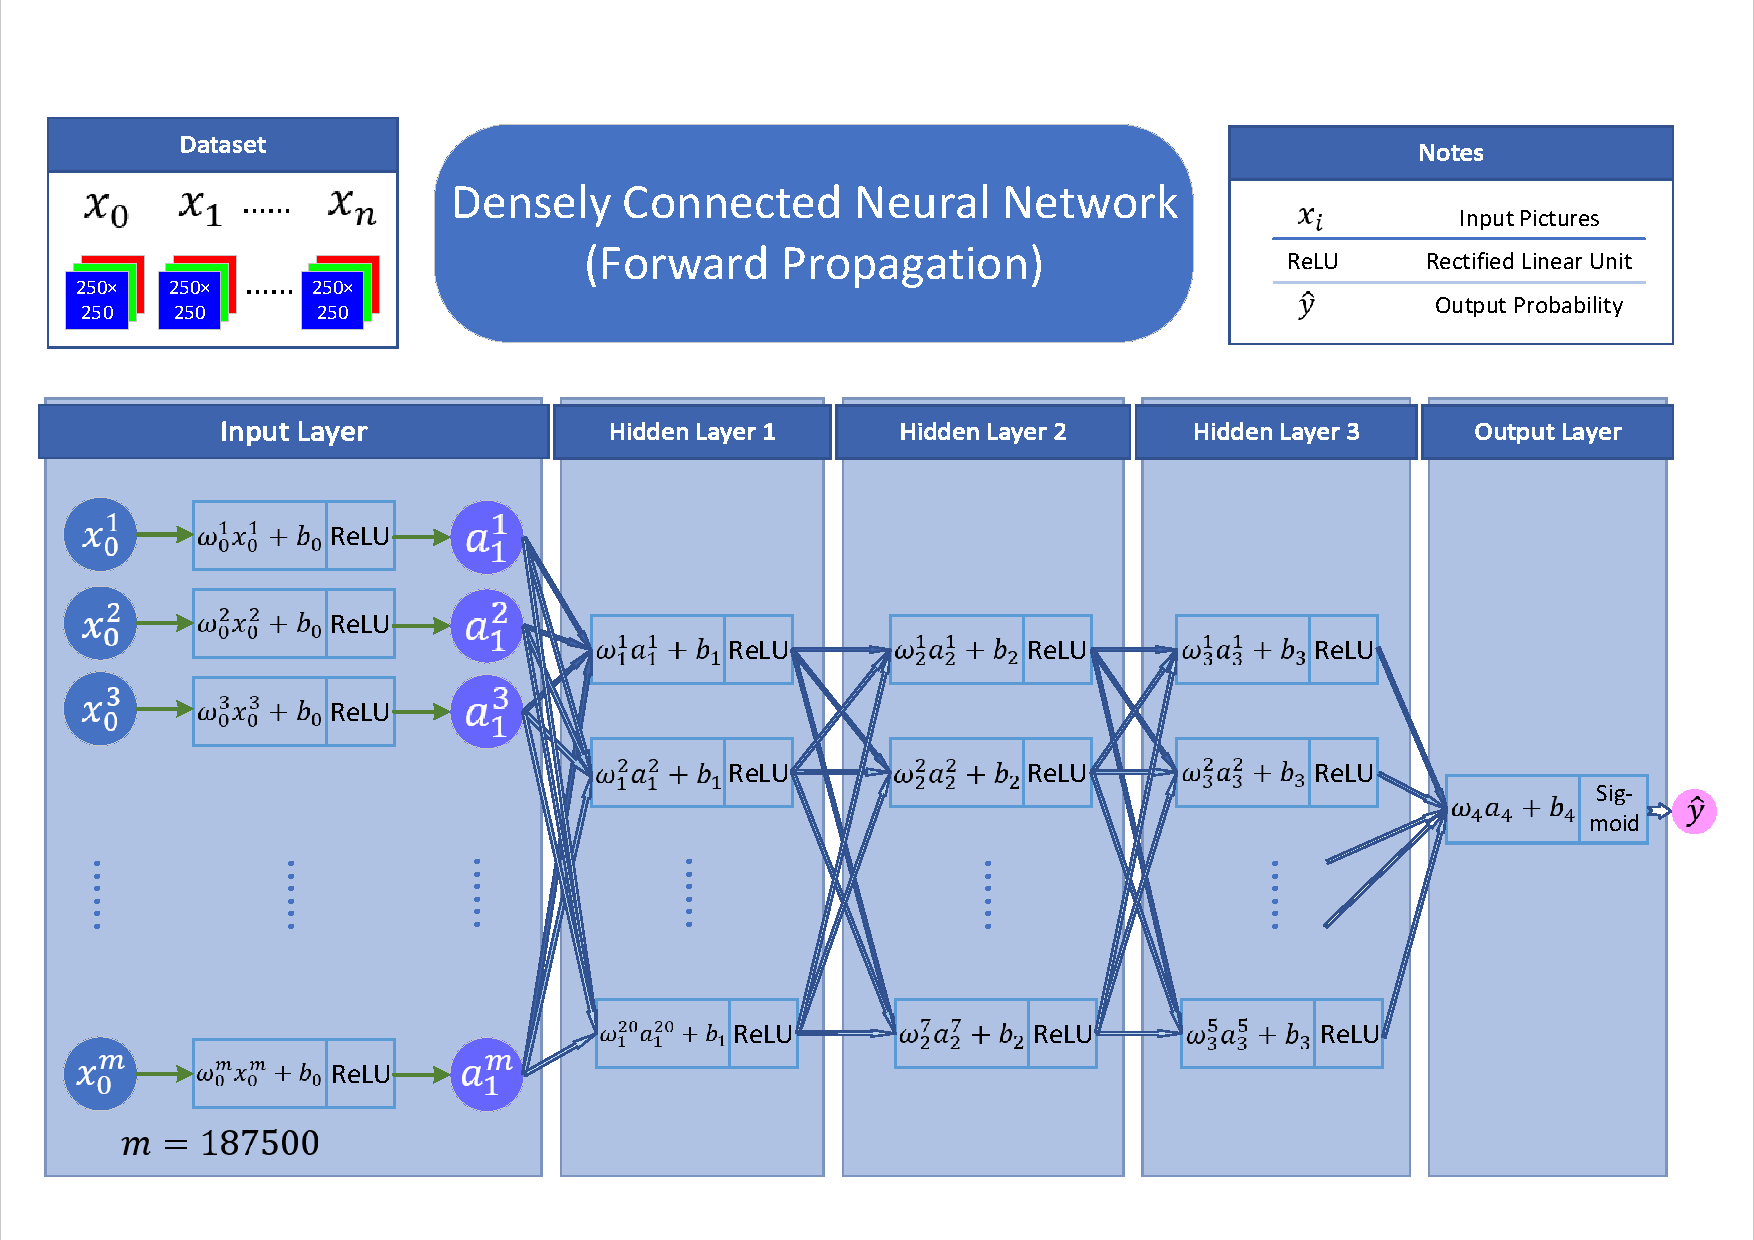
\includegraphics[width = 1\textwidth]{DCNN-F.pdf} 
	\caption{Basic Structure of DNN}
	\label{fig:DNN}
\end{figure}

Given the input $X_i$, which is the i th image of the training set, we can calculate the $z_{0}^{1} = \omega_{0}^{1} X_{i}^{1} + b_{0}^{1}$ where $\omega_{0}$ and $b_{0}$ are parameters of input layer and then apply ReLU function to all the 
linear unit z, which is $a_{1}^{1} = ReLU(z_{0}^{1})$ to eliminate the part of output of the first layer that is negative. 
After that do the same thing to the output of the input layer, then get the out put of hidden layers 1, 2, and 3. For the last layer which is also the output layer, the activation function is still the one we used before - the simoid function to get a possibility, which is the likelihood of a mistaken classification.
\paragraph{ }
The process of running the deep neural network: 
\begin{enumerate}
    \item randomly initialize the parameters of the deep neural network
    \item take the input then calculate the Loss function
    \item use back propagation to calculate the gradient of the parameters in the model
    \item use gradient decent algorithm to decrease the parameters along its gradient and update them in the network
    \item repeat the procedure until the loss function is small enough
\end{enumerate}

After the forward and backward propagation we will get a series of $\omega$ and $b$ to represent the neural network. Then try to use this model to classify a picture, the result $\hat{y}$ will be the possibility that the picture is a Vespa mandarinia.
\subsubsection{Introduction of Deep Neural Network to the Real Case} 
To use the Neural Network model to  predicts the likelihood of a mistaken classification, we choose to use the images provided in the dataset as input X, with some photos of Vespa mandarinia found from the Internet \cite{AGH}, 
We used 500 pictures with negative ID, and 200 pictures with real Vespa mandarinia as the training set, and 60 pictures as test set. After running the 
forward and backward propagation algorithm for 5000 times of iterations at a learning rate $\alpha = 0.0025$, the Loss decreases from  0.6075114409935868 to 0.08984676281165943. The cost function with respect to number of iterations is shown in the figure fig.\ref{fig:COSTFUNCTION}

\begin{figure}[!htbp]
	\centering
 	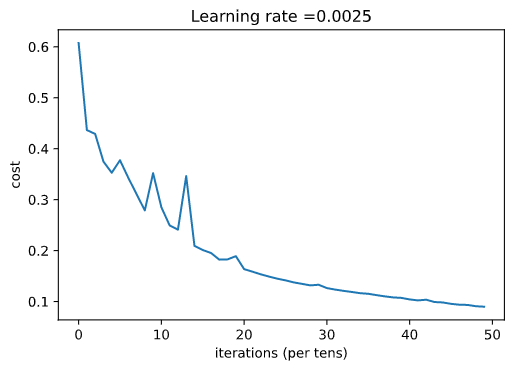
\includegraphics[width = 0.7\textwidth]{costFunction.png} 
	\caption{the curve of cost function with learning rate 0.0025}
	\label{fig:COSTFUNCTION}
\end{figure}

 By applying the model, we can predict the likelihood of a mistaken classification of the test set. The accuracy of this model to predict training set is 0.99857 while for the test set it is 0.80000. The result is satisfactory to predict the likelihood of a mistaken classification.



\section{Simulation Results}
\subsection{Problem1: The Prediction of Vespa Mandarinia's Spread Situation}
\subsubsection{Forecast of Vespa Mandarinia's Spread Situation after September in 2020 }
Although the spread situation of Vespa Mandarinia has been given, our model still did this part of simulation for testing purpose. And the results compared favorably with the practical ones.
\begin{figure}[!htbp]
	\centering
 	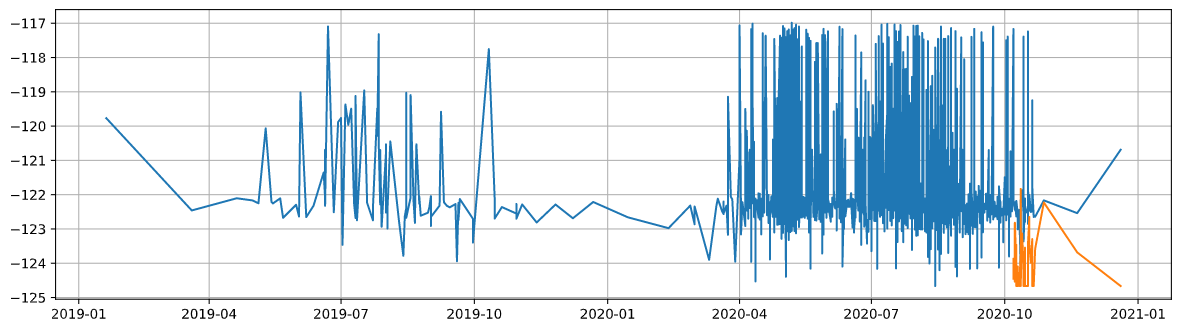
\includegraphics[width = 0.7\textwidth]{Longitude.png} 
	\caption{Forecast Data for Longitude}
	\label{fig:long}
\end{figure}

\begin{figure}[!htbp]
	\centering
 	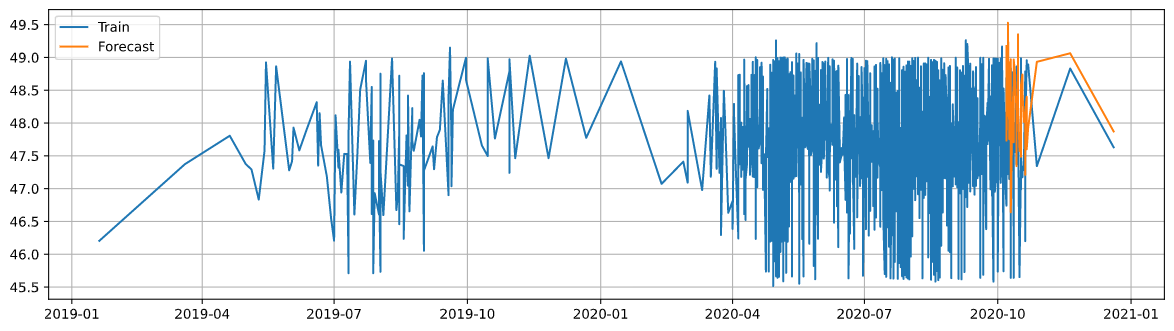
\includegraphics[width = 0.7\textwidth]{Latitude.png} 
	\caption{Forecast Data for Latitude}
	\label{fig:lat}
\end{figure}
Both figures show the original data and the forecast ones. The blue line represents the train set while the orange line shows the prediction results. Specifically, fig.\ref{fig:long} gives the information with respect to longitude and fig.\ref{fig:lat} gives the information about the latitude. The value for the lines are provided in the appendix, by tab.\ref{tab:PD2} respectively. From the figures, one can clearly tell that the forecast line matches the line that represents the train (reality) set with an acceptable error. This high-level correspondence implies the reliability of our model.

\subsubsection{Forecast of Vespa Mandarinia's Spread Situation in the Future}
Due to the limitation of the amount of given data and time, we predict 50 possible upcoming positive sightings and their locations with respect to longitude and latitude. The precision can be 
In order to visualize our results, we made a map (\ref{fig:map}) with all the possible locations marked as
\begin{figure}[!htbp]
	\centering
 	\includegraphics[width = 0.7\textwidth]{map.png} 
	\caption{Forecast Data}
	\label{fig:map}
\end{figure}
\subsubsection{Level of Precision}
This part is aimed at calculating the precision by terms of area in two dimensions, longitudinal and latitudinal. According to \textit{University Physics with Modern Physics (14th Edition)}, the radius of the earth is $R$, 6370 $km$ \cite{RN2}. Our assumption is that: the earth is a perfect sphere. Since the longitudinal and the latitudinal data have a precision of $10^{-3}$, we use the 0\# prediction data as an example. The latitude is $49.174^\circ$ and the longitude is $124.466^\circ$. 

The radius of the circle whose center passes the earth's axis and perpendicular to it can be calculated by Eq. (\ref{eq.9})
\begin{equation}
	r=R*sin(49.174^\circ)=4820km
	\label{eq.9}
\end{equation}
So the precision of longitudinal length is calculated by Eq. (\ref{eq.10})
\begin{equation}
	p_{long}=r*10^{-3}=4.82km
	\label{eq.10}
\end{equation}
And the precision of latitudinal length can be calculated by Eq. (\ref{eq.11})
\begin{equation}
	p_{lat}=R*\frac{2*49.174^\circ*10^{-3}}{360^\circ}=1.74km
	\label{eq.11}
\end{equation}
The precision results are summarized in the table Tab. \ref{tab:3}
\begin{table}[htbp]
\centering
\begin{tabular}{cc}
\hline
Item & Precision\\
\hline
Longitudinal length & 4.82 [km]\\
Latitudinal length & 1.74 [km]\\
Area & 8.388 [km^{2}]\\

\hline
\end{tabular}
\caption{Precision of the Prediction Model}
\label{tab:3}
\end{table}


\subsection{Problem2: The Prediction of the likelihood of a mistaken classification}



\subsection{Problem3: Prioritizing Upcoming Positive Sightings}

\subsection{Problem4: Update of Model with New Reports}

\subsection{Problem5: Evidence of the Eradication of Vespa Mandarinia in Washington State}

\section{Strengths and Weaknesses}
\subsection{Strengths}
\subsection{Weaknesses}

\section{Conclusions}

\section{Memorandum}

\bibliographystyle{plain}
\bibliography{newrefs}

\newpage

\begin{appendices}
\section{Code Example}
% \lstinputlisting[language=Matlab]{code/gene.m}
\section{Data for The Prediction of Vespa Mandarinia's Spread Situation}
\begin{table}[htbp]
\centering
\begin{tabular}{|l|l|l|l|l|l|}
\hline
Detection Date & Latitude    & Longitude    & Detection Date & Latitude    & Longitude    \\ \hline
2020/10/7      & 49.17027352 & -124.4655896 & 2020/10/15     & 49.34792642 & -124.665014  \\ \hline
2020/10/7      & 47.7265537  & -123.8828997 & 2020/10/15     & 48.27407842 & -124.665014  \\ \hline
2020/10/8      & 48.92301776 & -124.5513251 & 2020/10/16     & 47.56839839 & -124.665014  \\ \hline
2020/10/8      & 49.52368699 & -122.8407972 & 2020/10/17     & 47.69475221 & -124.665014  \\ \hline
2020/10/9      & 47.80090322 & -124.0750809 & 2020/10/17     & 47.49047502 & -124.6443257 \\ \hline
2020/10/9      & 47.75666786 & -123.9994218 & 2020/10/17     & 47.80283574 & -124.665014  \\ \hline
2020/10/9      & 48.39045254 & -123.485545  & 2020/10/17     & 47.69630331 & -124.665014  \\ \hline
2020/10/9      & 48.53449737 & -123.8621588 & 2020/10/17     & 47.94263189 & -123.7554979 \\ \hline
2020/10/9      & 48.64531332 & -124.665014  & 2020/10/17     & 47.4908341  & -124.3248868 \\ \hline
2020/10/10     & 48.96574578 & -124.665014  & 2020/10/17     & 48.18923916 & -124.1377971 \\ \hline
2020/10/10     & 46.94210441 & -124.0993169 & 2020/10/17     & 47.79149832 & -124.665014  \\ \hline
2020/10/10     & 46.63864391 & -124.3687582 & 2020/10/17     & 48.56991871 & -123.4814023 \\ \hline
2020/10/11     & 48.12809481 & -124.665014  & 2020/10/18     & 48.73790543 & -122.6697473 \\ \hline
2020/10/12     & 48.57361984 & -123.7789703 & 2020/10/18     & 48.51033619 & -123.477667  \\ \hline
2020/10/12     & 47.71539582 & -122.4873235 & 2020/10/19     & 48.01412082 & -123.9929558 \\ \hline
2020/10/12     & 47.79557506 & -121.8377628 & 2020/10/20     & 48.07388288 & -123.3061067 \\ \hline
2020/10/12     & 48.97493541 & -124.665014  & 2020/10/20     & 47.72954649 & -123.8207859 \\ \hline
2020/10/13     & 48.74424921 & -123.1520272 & 2020/10/20     & 47.20622806 & -124.42206   \\ \hline
2020/10/14     & 48.1082895  & -124.1282838 & 2020/10/20     & 48.15576865 & -124.665014  \\ \hline
2020/10/14     & 48.18329198 & -124.665014  & 2020/10/21     & 48.400179   & -124.665014  \\ \hline
2020/10/14     & 47.34359327 & -124.665014  & 2020/10/21     & 47.60545078 & -124.665014  \\ \hline
2020/10/14     & 48.36803272 & -124.2302224 & 2020/10/22     & 47.92866969 & -123.5968858 \\ \hline
2020/10/14     & 48.00750908 & -124.665014  & 2020/10/28     & 48.93044592 & -122.2387128 \\ \hline
2020/10/15     & 48.37186873 & -124.665014  & 2020/11/20     & 49.06401576 & -123.7006217 \\ \hline
2020/10/15     & 48.57671937 & -123.5548522 & 2020/12/20     & 47.8645205  & -124.665014  \\ \hline
\end{tabular}
\caption{Corresponding Prediction Data for the Spread of Vespa Mandarinia in 2020 after September}
\label{tab:PD2}
\end{table}


\begin{table}[htbp]
\centering
\begin{tabular}{|l|l|l|l|l|l|}
\hline
   & Latitude    & Longitude    &    & Latitude    & Longitude    \\ \hline
0  & 49.17403896 & -124.4538782 & 25 & 49.35229792 & -124.665014  \\ \hline
1  & 47.73191804 & -123.8656101 & 26 & 48.27739322 & -124.665014  \\ \hline
2  & 48.92776934 & -124.5379701 & 27 & 47.57461443 & -124.665014  \\ \hline
3  & 49.52857255 & -122.820109  & 28 & 47.69417562 & -124.665014  \\ \hline
4  & 47.8089629  & -124.0617151 & 29 & 47.49565803 & -124.6359059 \\ \hline
5  & 47.75334323 & -123.9821008 & 30 & 47.8024512  & -124.665014  \\ \hline
6  & 48.39041011 & -123.4646326 & 31 & 47.70182486 & -124.665014  \\ \hline
7  & 48.54064151 & -123.8544132 & 32 & 47.94729325 & -123.7408797 \\ \hline
8  & 48.65106622 & -124.665014  & 33 & 47.48572791 & -124.3141035 \\ \hline
9  & 48.97113468 & -124.665014  & 34 & 48.19347846 & -124.1223144 \\ \hline
10 & 46.94173059 & -124.093804  & 35 & 47.79948029 & -124.665014  \\ \hline
11 & 46.63927408 & -124.3544156 & 36 & 48.56901654 & -123.4709612 \\ \hline
12 & 48.12898984 & -124.665014  & 37 & 48.73887906 & -122.6501231 \\ \hline
13 & 48.57397937 & -123.7606421 & 38 & 48.51365724 & -123.4670535 \\ \hline
14 & 47.7065885  & -122.4762115 & 39 & 48.01706091 & -123.9848345 \\ \hline
15 & 47.79404092 & -121.8308073 & 40 & 48.0727181  & -123.2949466 \\ \hline
16 & 48.96925442 & -124.665014  & 41 & 47.72756975 & -123.8165881 \\ \hline
17 & 48.74060346 & -123.1334024 & 42 & 47.210642   & -124.4159169 \\ \hline
18 & 48.11014386 & -124.1108326 & 43 & 48.15805177 & -124.665014  \\ \hline
19 & 48.18721999 & -124.665014  & 44 & 48.40140542 & -124.665014  \\ \hline
20 & 47.3429613  & -124.665014  & 45 & 47.599517   & -124.665014  \\ \hline
21 & 48.36574067 & -124.2340001 & 46 & 47.9300033  & -123.5793421 \\ \hline
22 & 48.01000657 & -124.665014  & 47 & 48.93275896 & -122.2284755 \\ \hline
23 & 48.38053269 & -124.665014  & 48 & 49.06355217 & -123.6829364 \\ \hline
24 & 48.58172284 & -123.5452854 & 49 & 47.8714681  & -124.665014  \\ \hline
\end{tabular}
\caption{Prediction Data for the Spread of Vespa Mandarinia}
\label{tab:PD1}
\end{table}



\end{appendices}
\end{document}

